\documentclass[11pt,a4paper]{article}
\usepackage[T1]{fontenc}
\usepackage[margin=1in]{geometry}
\usepackage{amsmath,amssymb,mathtools}
\usepackage{booktabs}
\usepackage{graphicx}
\usepackage{xcolor}
\usepackage[colorlinks=true,linkcolor=blue!60!black,citecolor=blue!60!black,urlcolor=blue!60!black]{hyperref}
\usepackage{microtype}
\usepackage{xurl}
\setlength{\emergencystretch}{3em}
\usepackage{enumitem}
\usepackage[most]{tcolorbox}
\newtcolorbox{keybox}[1][]{colback=blue!3,colframe=blue!45!black,boxrule=0.5pt,left=4pt,right=4pt,top=3pt,bottom=3pt,#1}
\newtcolorbox{failbox}[1][]{colback=red!3,colframe=red!45!black,boxrule=0.5pt,left=4pt,right=4pt,top=3pt,bottom=3pt,#1}
\hypersetup{pdftitle={Gated exciton fluids V},pdfauthor={Xavier Callens},pdfsubject={Three dimensions: what the T-duality, holography and projection analogies do and do not give}}

\begin{document}
\begin{center}
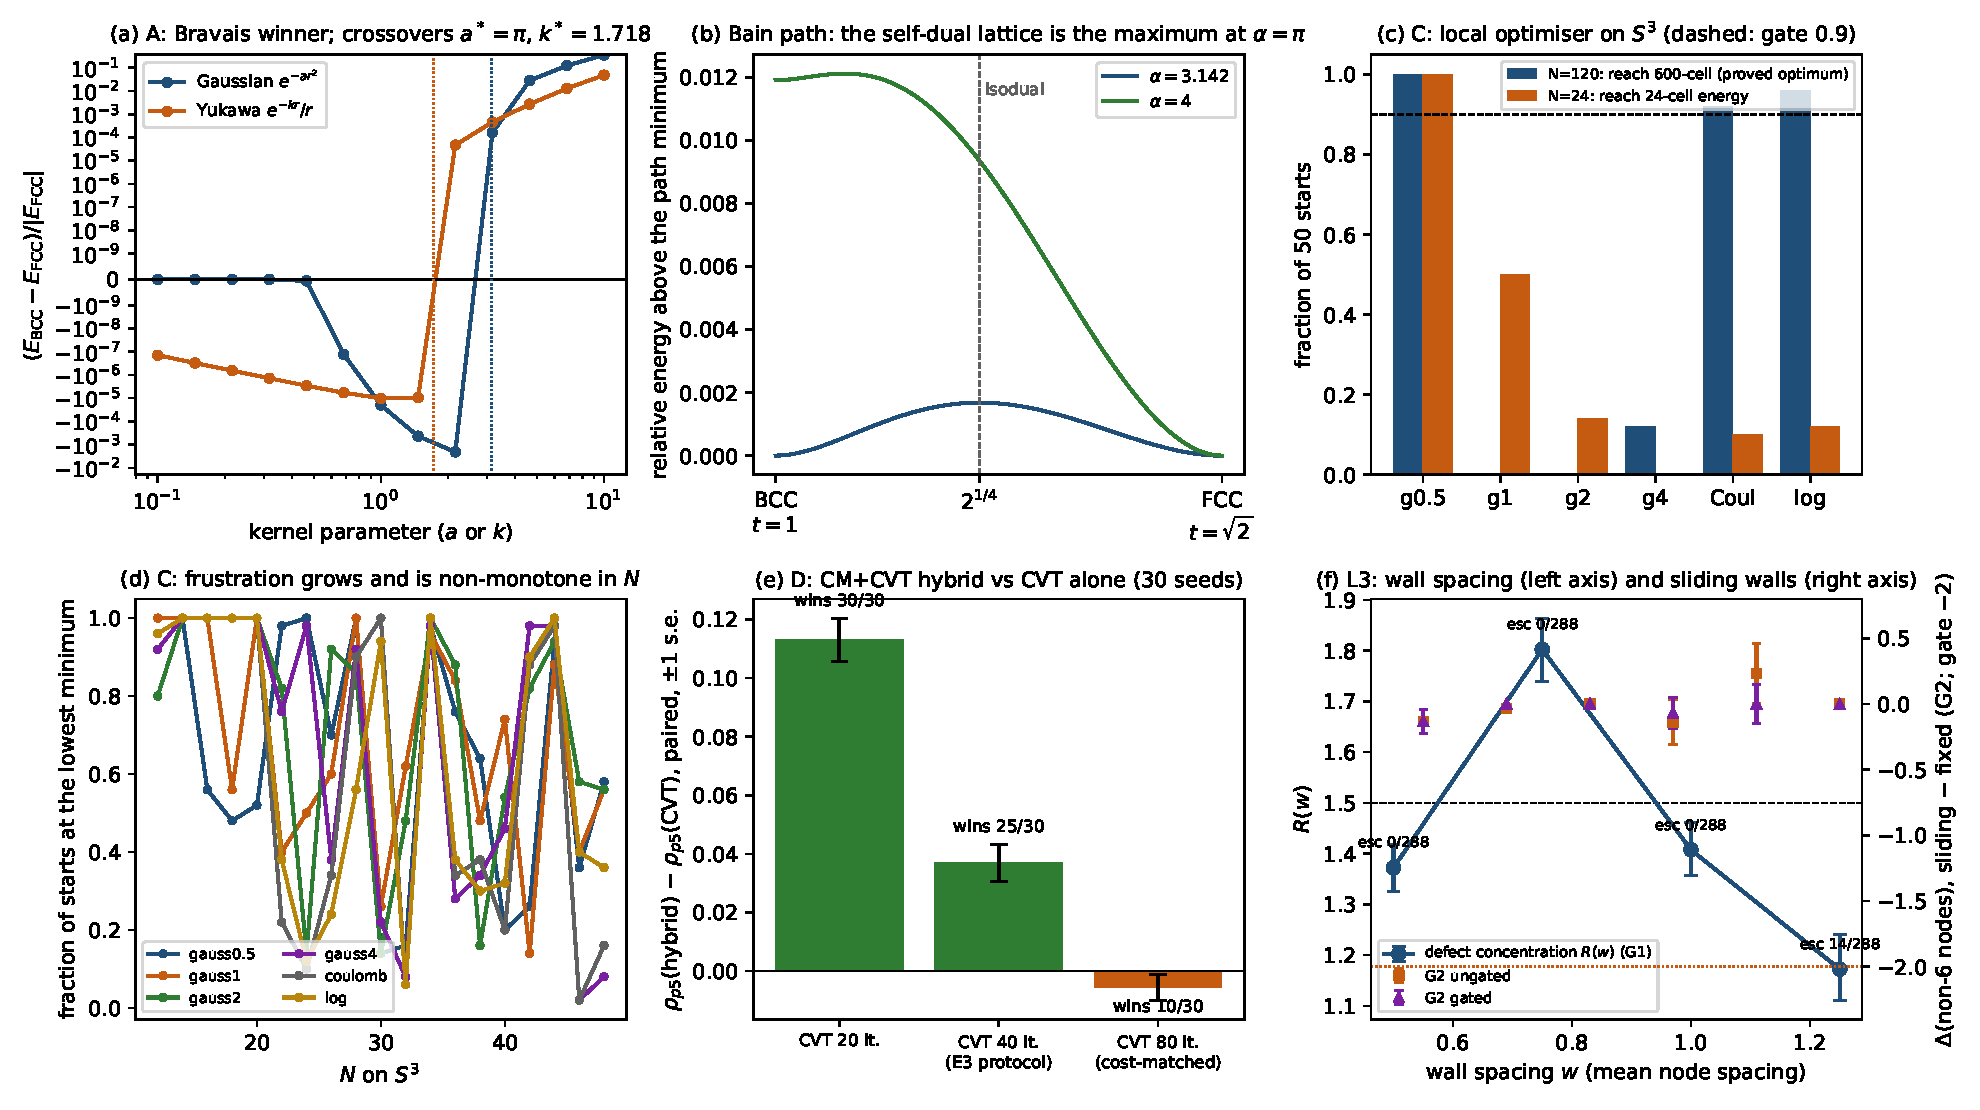
\includegraphics[width=0.98\textwidth]{figs_companion5/fig_round1.pdf}\\[2pt]
{\footnotesize (a) Which Bravais lattice wins in 3D for Gaussian and Yukawa kernels at unit density; the crossovers are $a^*=\pi$
(exact, Poisson duality) and $k^*=1.718$. (b) Gaussian energy along the Bain path between BCC and FCC: at the self-dual point
$\alpha=\pi$ the self-dual (isodual) lattice is the \emph{maximum}. (c) Fraction of 50 random starts that a local optimiser brings
to the proved optimum on $S^3$ (600-cell, $N=120$) and to the 24-cell energy ($N=24$). (d) Fraction of starts reaching the lowest
minimum found, $N\le 48$ on $S^3$. (e) Hybrid CM$+$CVT mesh against CVT alone, paired over 30 seeds. (f) Wall-spacing scan and
sliding walls in the Fenris container study.}
\end{center}
\vspace{-0.6em}
\begin{center}
{\Large\textbf{Gated exciton fluids V:}\\[2pt]
\large three dimensions --- what the T-duality, holography and projection analogies\\ do and do not give, measured}\\[8pt]
Xavier Callens\\ {\small SocrateAI Research \quad\url{https://github.com/xaviercallens/SocrateAI-Scientific-QuantumFluids}}\\[2pt]
{\small October 2026 \quad (version 2: adds H1$'$; version 3: adds H1$''$ and H1$'''$, certified bounds)}
\end{center}
\vspace{-0.4em}

\begin{abstract}\small\noindent
Papers~I--IV~\cite{CallensI,CallensII,CallensIII,CallensIV} proved that the gated dipole kernel is completely monotone in $r^2$ and
tested, negatively, three heuristics for the two-dimensional node problem. This paper turns to three dimensions, where the owner
asked whether ideas borrowed from string theory --- lifting to 8 or 24 dimensions, holography, projection, T-duality --- could
``solve'' the problem. We first state the known fact that reframes the question: in $\mathbb R^3$ no configuration is universally
optimal, because the Poisson dual of FCC is BCC and the two exchange roles at the self-dual Gaussian parameter $\alpha=\pi$; the
open problems are the Gaussian-core conjecture (FCC/BCC among \emph{all} configurations), crystallisation, and mixed kernels.
We then report pre-registered experiments. Round~1: among 3D Bravais lattices the minimiser is always FCC or BCC (29/29 kernel
points; crossovers $a^*=\pi$ to $3\times10^{-14}$ and $k^*=1.7179$ for Yukawa); random-restart searches over non-Bravais cells with
up to 16 points find nothing below $\min(\mathrm{FCC},\mathrm{BCC},\mathrm{HCP},\mathrm{A15})$ in 9\,860 restarts; on $S^3$, where the
600-cell is a \emph{proved} optimum, a local optimiser reaches it in 46--50 of 50 starts for Coulomb, logarithmic and soft Gaussian
kernels but in 0 and 6 of 50 for stiffer Gaussians; a completely-monotone pre-relaxation improves a CVT mesh only when the CVT is
given less work; sliding container walls reduce the defect count in 0 of 6 shapes. A direct computation along the Bain path shows
that at $\alpha=\pi$ the self-dual (isodual) 3D lattice is the energy \emph{maximum} between the two degenerate minima: the
T-duality analogy explains why no universal optimum exists in 3D rather than pointing to one. The mode-sum (``Kaluza--Klein tower'')
evaluator of the gated kernel is 4--7 times cheaper than a tail-corrected image sum. Round~2 is negative throughout: an
$\alpha$-homotopy from a soft kernel reaches the proved 600-cell in 0, 0 and 6 of 50 seeds at $a=1,2,4$, while plain restarts at equal compute reach it in 50/50 at $a=4$ (it does help for the 24-cell), so by the
registered rule our 3D searches are declared unreliable; Gaussian mixtures straddling the self-dual point produce nothing below
FCC/BCC/HCP in 5\,100 restarts; a search for formally self-dual configurations accepts nothing, but its objective cannot tell the
known one (diamond) from configurations $10^{-3}$ away, so the negative is uninformative; and the two-point linear-programming
code failed its own one-dimensional sanity gate (under an admissibility tolerance fixed in code, not registered) and was therefore
not run in $d=3$. \emph{Version~2} adds H1$'$: the $\alpha=\pi$ question of H1 turned out to be answered in the literature
(two-point bound $0.2232$ against $0.2315$ in $d=3$); after an attempt at rigorous certificates was abandoned in development, a
re-registered \emph{numerical, not certified} run reproduces the published $d=1,2,3$ values within the registered windows and
gives gaps of $0.48\%$, $6.7\%$ and $21.6\%$ below the best lattice in $d=3$ at $\alpha=2,4,8$: numerically, at polynomial
degree $\le40$ and with the best lattice as reference, two-point bounds do not settle the 3D question at any $\alpha$ tested.
\emph{Version~3} adds interval-certified bounds (256-bit interior point, exact cutting planes, arb certificate): at $K=40$
(polynomial degree $39$) the $d=3$, $\alpha=\pi$ gate failed by $3\times10^{-8}$ (H1$''$); at $K=50$ (degree $49$) it passed
(H1$'''$, certified $0.2232178194$ against the published $0.22321782$), and the certified lower bounds at $\alpha=2,4,8$ lie
$0.48\%$, $6.7\%$ and $21.6\%$ below the best lattice. The bound values are rigorous; that two-point bounds cannot do better
remains numerical. A review found a defect in our certificate code (sub-ulp negative intervals of $\hat f$ not checked); an
independent re-check confirms every reported bound, one of them ($K=60$, not a gate) only after adding a small lift. Everything is small-scale, classical and
single-engine; nothing uses the unrefereed planar lattice theorem; written with an AI system and not refereed.
\end{abstract}

\section{The question, restated}\label{sec:restate}

For a unit-density lattice $L\subset\mathbb R^3$ and the Gaussian kernel $e^{-\alpha r^2}$, Poisson summation gives
$\theta_L(\alpha)=\sum_{v\in L\setminus0}e^{-\alpha|v|^2}$ and $1+\theta_L(\alpha)=(\pi/\alpha)^{3/2}\,(1+\theta_{L^*}(\pi^2/\alpha))$.
The dual of FCC is BCC. Hence $\theta_{\rm FCC}(\pi)=\theta_{\rm BCC}(\pi)$ exactly, BCC is lower for $\alpha<\pi$ and FCC for
$\alpha>\pi$ (Fig.~(a); our lattice search finds the crossover at $a^*=3.14159265358987$). By Bernstein's theorem every completely
monotone kernel is a positive mixture of Gaussians, so no single configuration can minimise all of them: \textbf{universal
optimality is false in $\mathbb R^3$ for every configuration}. This is known~\cite{CK07,CKS09}; we state it because it voids the
phrase ``solve the Cohn--Kumar conjecture in 3D''. What is open in three dimensions is
\begin{enumerate}[leftmargin=1.6em,itemsep=1pt]
\item[Q1] the Gaussian-core conjecture: BCC ($\alpha<\pi$) and FCC ($\alpha>\pi$) minimise among \emph{all} periodic configurations
(``no proof is known''~\cite{CKS09}); at $\alpha=\pi$ itself the lowest known energy (``putative ground state'') is a Maxwell coexistence of the two at densities
$0.99899854\le\rho\le1.00100312$, about $4\times10^{-6}$ below either pure lattice~\cite{CKS09};
\item[Q2] crystallisation (periodicity of minimisers) for soft repulsions;
\item[Q3] kernels whose Bernstein measure charges both sides of $\pi$, for which nothing excludes a non-Bravais minimiser.
\end{enumerate}
``Borrowing from 8D/24D'' can therefore only mean borrowing \emph{proof mechanisms} --- self-duality, Fourier interpolation,
linear-programming bounds --- not answers. The experiments below give each analogy a falsifiable form.

\begin{keybox}
\textbf{What was pre-registered.} Round~1 (\texttt{exploration/exciton/three\_d/PREREG.md}, commit \texttt{357ee6d}): A (Bravais),
B (non-Bravais cells), C ($S^3$), D (hybrid mesh); L3 (\texttt{fenris-gated/L3\_PREREG.md}, see the caveat in \S\ref{sec:L3});
L1 (\texttt{exploration/exciton/kk/PREREG.md}). Round~2 (\texttt{PREREG\_round2.md}, commit \texttt{51a85b1}): F1, T2, T1, H1.
Version~2: H1$'$ (\texttt{three\_d/H1p/PREREG.md}, \texttt{d668109}; amendments A1 \texttt{83a3500}, A2 \texttt{968dd32}, both before
any gate run, but A2's acceptance tolerance and windows were set after H1's outcomes were known).
Version~3: H1$''$ (\texttt{three\_d/H1pp/PREREG.md}, \texttt{b1d2de5}) and H1$'''$ (\texttt{three\_d/H1ppp/PREREG.md},
\texttt{1e50f4b}; evaluator replaced during the runs, \texttt{162dfc3}, see \texttt{H1ppp/DEVIATIONS.md}).
All gates, restart counts and thresholds were fixed before the runs; deviations are dated in each \texttt{RESULTS.md} and
summarised in \S\ref{sec:process}. An independent adversarial review preceded this write-up; its corrections are applied and
listed.
\end{keybox}

\section{Round 1}

\subsection{A: Bravais lattices}
Free 9-parameter unit-volume cell with periodic Minkowski re-reduction, 300 random starts per kernel point, Ewald energies with
tails $\le8\times10^{-16}|E|$; kernels Gaussian ($a\in$ 13 log-spaced points in $[0.1,10]$), Yukawa ($k$, same grid), Riesz
($s\in\{4,6,12\}$). Gate A1 (global Bravais minimiser $=$ lower of FCC/BCC at $\ge95\%$ of points): \textbf{met, 29/29}. Five Gaussian
points ($a\le0.46$) are degenerate in double precision (FCC, BCC, A15, C15 and diamond agree to $10^{-9}$), so the pass is
vacuous there; 24/29 non-degenerate points still exceed 95\%. Crossovers: Gaussian $a^*=\pi$ (exact by duality), Yukawa
$k^*=1.7179$ with a relative gap of only $10^{-7}$--$10^{-5}$ around it, Riesz FCC throughout $s\in[3.05,30]$. Verification:
analytic gradients against finite differences ($2\times10^{-9}$), Gaussian energies against closed-form theta functions
($\le3\times10^{-13}$), Yukawa/Riesz against brute-force sums with continuum tails and an independent Ewald code ($10^{-15}$).

\subsection{B: non-Bravais cells}
$N\in\{2,4,8,12,16\}$ points per free cell; 100 restarts for $N\le4$, 60 for $N=8$, 40 for $N=12,16$ (reduced from the registered
100 for time; disclosed). References FCC, BCC, HCP, diamond, A15 (all representable at the relevant $N$), C15 ($N=12$ only).
Gate B1 (restarts reach the best reference in $\ge50\%$ of cases for $N\le4$, $\ge10\%$ for $N=16$): \textbf{not met for
$N\le4$ under the strictest reading} (49/58 gated cells pass; the 9 failures sit at 39--49\%, all near the FCC/BCC crossovers
where the two basins compete; the median hit fraction, 0.76 at $N=2$ and 0.66 at $N=4$, would pass a pooled reading); met for
$N=16$ (29/29, minimum 25\%). Gate B2 (discovery): \textbf{nothing} below $\min(\mathrm{FCC},\mathrm{BCC},\mathrm{HCP},\mathrm{A15})$
by more than $10^{-8}$ in 9\,860 restarts over 145 cells. A relaxed HCP/DHCP stacking scan is never below FCC/BCC by more than
$10^{-9}$, consistent with the statement that FCC is the best Barlow packing for the low-density Gaussian core~\cite{CK08}.
The first A runs were invalid (a determinant-sign bug, two overlapping runs, a hang on skewed cells); their records are kept in
\texttt{run0\_buggy/} and the reported numbers are the fourth run.

\subsection{C: a proved control on $S^3$}\label{sec:C}
$N$ points on the unit $S^3$, chordal kernels $e^{-a d^2}$ ($a\in\{0.5,1,2,4\}$), $1/d$ and $\log(1/d)$; L-BFGS-B from 50 random
starts per kernel. The 600-cell is universally optimal for $N=120$~\cite{CK07}, a \emph{proved} target. Gate C1 ($\ge45/50$ starts
within $10^{-8}$ of $E_{600}$ for every kernel): \textbf{not met}. Success 50/50 ($a=0.5$), 46/50 (Coulomb), 48/50 (log), 6/50
($a=4$, 44 starts end $10^{-3}$ above; round~2 indicates a low draw: restarts of the same optimiser succeed in 1\,916 of 5\,790 runs, fresh starts in 38/140, Sec.~\ref{sec:F1}), 0/50 ($a=2$, all converge to a family of local minima $7\times10^{-6}$ above). For $a=1$ all
50 starts hit the registered 8\,000-iteration cap $2$--$3\times10^{-8}$ above $E_{600}$; the review asked for a rerun with the cap
raised to 150\,000: all converge ($16\,640$--$66\,673$ iterations) at $1.5$--$2.1\times10^{-8}$ above, and two polished configurations
have minimum chord $0.50$ against $0.618$ for the 600-cell with a distance-spectrum deviation of $0.22$ --- \emph{distinct local
minima}, not the 600-cell with residual error, in a landscape so flat that the best local minima lie within $2\times10^{-8}$ of
the proved optimum. No start went below $E_{600}$. For $N=24$ the 24-cell energy is reached in 50, 25, 7, 0, 5, 6 of 50 starts
(same kernel order); the 24-cell is known \emph{not} to be universally optimal and to have a small basin of attraction~\cite{CCEK07},
and our Coulomb and log runs reproduce the latter qualitatively with a different potential. Frustration scan: a second
distinct minimum appears at $N=12$ (stiff Gaussians, Coulomb, log), 16 ($a=0.5$), 18 ($a=1$); non-uniqueness is common from
$N=22$ and non-monotone in $N$ (Fig.~(d)). Seeds for $(N=120,\ \text{kernel }0)$ and $(N=20,\ \text{kernel }1)$ coincide (a formula
artefact; correlated, not independent, streams).

\begin{failbox}
\textbf{Reading.} Where the optimum is proved and the kernel is long-ranged or soft, a plain local optimiser finds it; where the
kernel is stiffer it is trapped. The obstacle of the three-dimensional problem in our hands is the landscape, not the dimension.
Any method that claims to help in 3D must first pass this control; round~2 (F1) is built on it.
\end{failbox}

\subsection{D: a CM pre-relaxation as a mesh accelerator}
Continuation of E3 of paper~IV with the same $N=216$ periodic cube and the registered 30 seeds: CM relaxation followed by 20 Lloyd
iterations against CVT alone. ``Equal total iterations'' had not been defined in the pre-registration; the run's author fixed
CVT-40 as primary before running and added CVT-20 and CVT-80 as sensitivity arms. Hybrid median 5th-percentile radius ratio
$0.7057$: against CVT-40 (the E3 protocol) $+0.0370\pm0.0063$, wins 25/30; against CVT-20 $+0.113\pm0.007$, 30/30; against
CVT-80, the \emph{cost-matched} arm (CM stage $\approx60$\,s, hybrid $\approx82$\,s, CVT-80 $\approx88$\,s), $-0.0055\pm0.0045$,
wins 10/30. \textbf{Verdict: met against CVT-20/40, not met at matched cost}; the hybrid is a convergence accelerator at best. It
does not improve the worst element (worst $\rho$ 0.014 vs 0.029, worst minimum dihedral $0.73^\circ$ vs $1.44^\circ$). Seed 0 was a
development seed inside the registered set; without it, $+0.0371\pm0.0065$, 24/29.

\subsection{L3: wall spacing and sliding walls in the Fenris study}\label{sec:L3}
A fresh clone of \texttt{rusty-Fenris-CMRR} (commit \texttt{6d0df125}, never pushed) with the kernel patch of paper~III. G1
(wall-spacing scan $w\in\{0.5,0.75,1,1.25\}$, random-sequential-addition starts, 6 shapes $\times$ 2 kernels $\times$ 24 starts):
0/288 escapes at $w\le1$, 14/288 at $w=1.25$. \textbf{The registered $w=1$ wall confines with RSA starts}, so the ``did not confine''
finding of paper~III came from the uniform starts, not from the spacing; the saddle mechanism was not tested. Defect concentration
$R(w)=1.37,1.80,1.41,1.17$; the registered threshold $1.5$ is met only at $w=0.75$ and that value is confounded by the
triangulation-site rule (all wall nodes used as sites at $w\ne0.5$). G2 (engine-level sliding walls, $w=0.5$, 30 paired starts per
shape): \textbf{0 of 6 shapes} reach a decrease of 2 defects for either kernel (square $-0.13\pm0.09$, rect $-0.14\pm0.17$,
L-shape $+0.23\pm0.23$, others $\approx0$); the wall moves by at most $0.05$; the wall-coordinate L-BFGS hit its 40-iteration cap in
25--30 of 30 starts for two shapes, so this is weak evidence for those shapes. Compared with E2 of paper~IV (joint minimisation from
the start) the square has the same sign and a 15 times smaller magnitude. \emph{Caveat:} \texttt{L3\_PREREG.md} was untracked when
the runs were made; its registration time rests on the author's attestation, not on git.

\subsection{L1: the Kaluza--Klein tower as an evaluator}
The gated kernel of paper~I is $U(r)=\frac{4}{\ell}\sum_{m\ge1}(\varphi_m(z_e)-\varphi_m(z_h))^2K_0(m\pi r/\ell)$, a mode sum with
exponentially decaying terms, or an image sum with algebraic tails. On four parameter sets and $10^4$ random $r\in[0.3d,6\ell]$ the
adaptive mode sum (binned in $r$) costs $0.028$--$0.036$\,s against $0.148$--$0.191$\,s for the image sum with an Euler--Maclaurin
tail ($N=60$), i.e. $4.1$--$6.7\times$ ($\ge5\times$ on 2 of 4 sets, the registered target); the image sum is accurate to $10^{-12}$
only for $r\lesssim1.1$--$1.9\,\ell$ because of cancellation. Gate G1 met with a disclosed caveat (mpmath reference at 10 points per
set, float modal sum as reference elsewhere, $7.8\times10^{-16}$ agreement), G2 partial; the Rust crate was therefore not built. The
``KK tower'' is real and useful, and it is exactly Prop.~2 of the mathematical note.

\section{The T-duality analogy, computed}\label{sec:bain}
In the three cases where universal optimality is known or conjectured ($A_2$ up to similarity, $E_8$, $\Lambda_{24}$) the
minimiser is a fixed point of Poisson duality. Along the body-centred-tetragonal (Bain) path $\mathrm{bct}(t)$, $c/a=t$, unit
density, $t=1$ is BCC, $t=\sqrt2$ is FCC, and the dual of $\mathrm{bct}(t)$ is similar to $\mathrm{bct}(\sqrt2/t)$; the fixed point
$t=2^{1/4}$ is isodual. Direct summation (tails $<10^{-30}$; \texttt{AB/bain\_selfdual.py}):
\begin{center}\small
\begin{tabular}{lcccc}\toprule
$\alpha$ & $E(\mathrm{BCC})$ & $E(\mathrm{FCC})$ & $E(\text{isodual})$ & extremum on the path\\\midrule
$\pi$ & 0.231536266184 & 0.231536266184 & 0.231925337063 & \textbf{maximum at $t=2^{1/4}$}\\
2.5 & 0.526007 & 0.527283 & 0.527031 & minimum at BCC\\
4 & 0.078896 & 0.077968 & 0.078697 & minimum at FCC\\\bottomrule
\end{tabular}
\end{center}
The symmetry $t\leftrightarrow\sqrt2/t$ holds to $10^{-16}$. \textbf{At the self-dual point the self-dual lattice is the worst
point of the path}: the duality symmetry is broken into two degenerate minima exchanged by it, the opposite of dimensions 8 and
24. T-duality thus explains the absence of a universal optimum in 3D; it designates no candidate. What survives of the analogy is
\emph{formal duality} in the sense of~\cite{CKS09}: the diamond structure $D_3^+$ is formally self-dual, and the question whether
any formally self-dual configuration beats FCC/BCC at $\alpha=\pi$ is the content of T1 (\S\ref{sec:round2}). Averaged holography
over the Narain moduli space gives, by the Siegel mean-value theorem, the \emph{average} Gaussian energy over unimodular lattices,
$(\pi/\alpha)^{3/2}-1$, never the minimum; it is not a tool for this problem.

\section{The holography analogy, stated as a question}
The proof of universal optimality in dimensions 8 and 24~\cite{CKMRV22} is holographic in a precise sense: a radial Schwartz function
is reconstructed from its values and Fourier values (and derivatives) at the radii $\sqrt{2n}$, through modular forms of level
one. In $d=3$ a radial function is an odd function of the line, and the interpolation nodes $\pm\sqrt n$ of~\cite{RV19} are the
norms of $\mathbb Z^3$ --- self-dual, but a poor minimiser. \emph{Does a radial Fourier interpolation formula exist in $d=3$ with the
FCC norms as nodes for $f$ and the BCC norms as nodes for $\hat f$?} We have not found this question in the literature and leave it
to specialists; even if it exists it cannot prove universal optimality (false), but it could certify FCC at a given $\alpha$ through
the linear-programming bound. What we can compute is the size of the two-point LP gap in $d=3$ (H1, \S\ref{sec:round2}; numerical values in version~2, \S\ref{sec:h1p}).

\section{Round 2}\label{sec:round2}
% Round 2 of paper V. Sources: exploration/exciton/three_d/{F1,T12,H1}/RESULTS.md (pre-registration PREREG_round2.md, 51a85b1).
\begin{failbox}
\textbf{Round 2 in one paragraph.} F1: the $\alpha$-homotopy reaches the proved $S^3$ optimum (600-cell, $N=120$) in
\textbf{F1HOMA} of 50 seeds at $a=1,2,4$, so gate F1a fails at every $a$ and the registered stop rule applies: the structure
searches of this programme are declared unreliable. T2: no structure below FCC/BCC/HCP for Gaussian mixtures straddling the
self-dual point (0 candidates in 75 cells, 5\,100 restarts). T1: no formally self-dual configuration accepted --- but the search
cannot distinguish the known one (diamond) from configurations $10^{-3}$ away, so this negative carries no information. H1: the
linear-programming code failed its own sanity gate in $d=1$ at $\alpha=\pi$ (under an admissibility tolerance fixed in code,
not registered) and was therefore not run in $d=3$.
\end{failbox}

\begin{center}
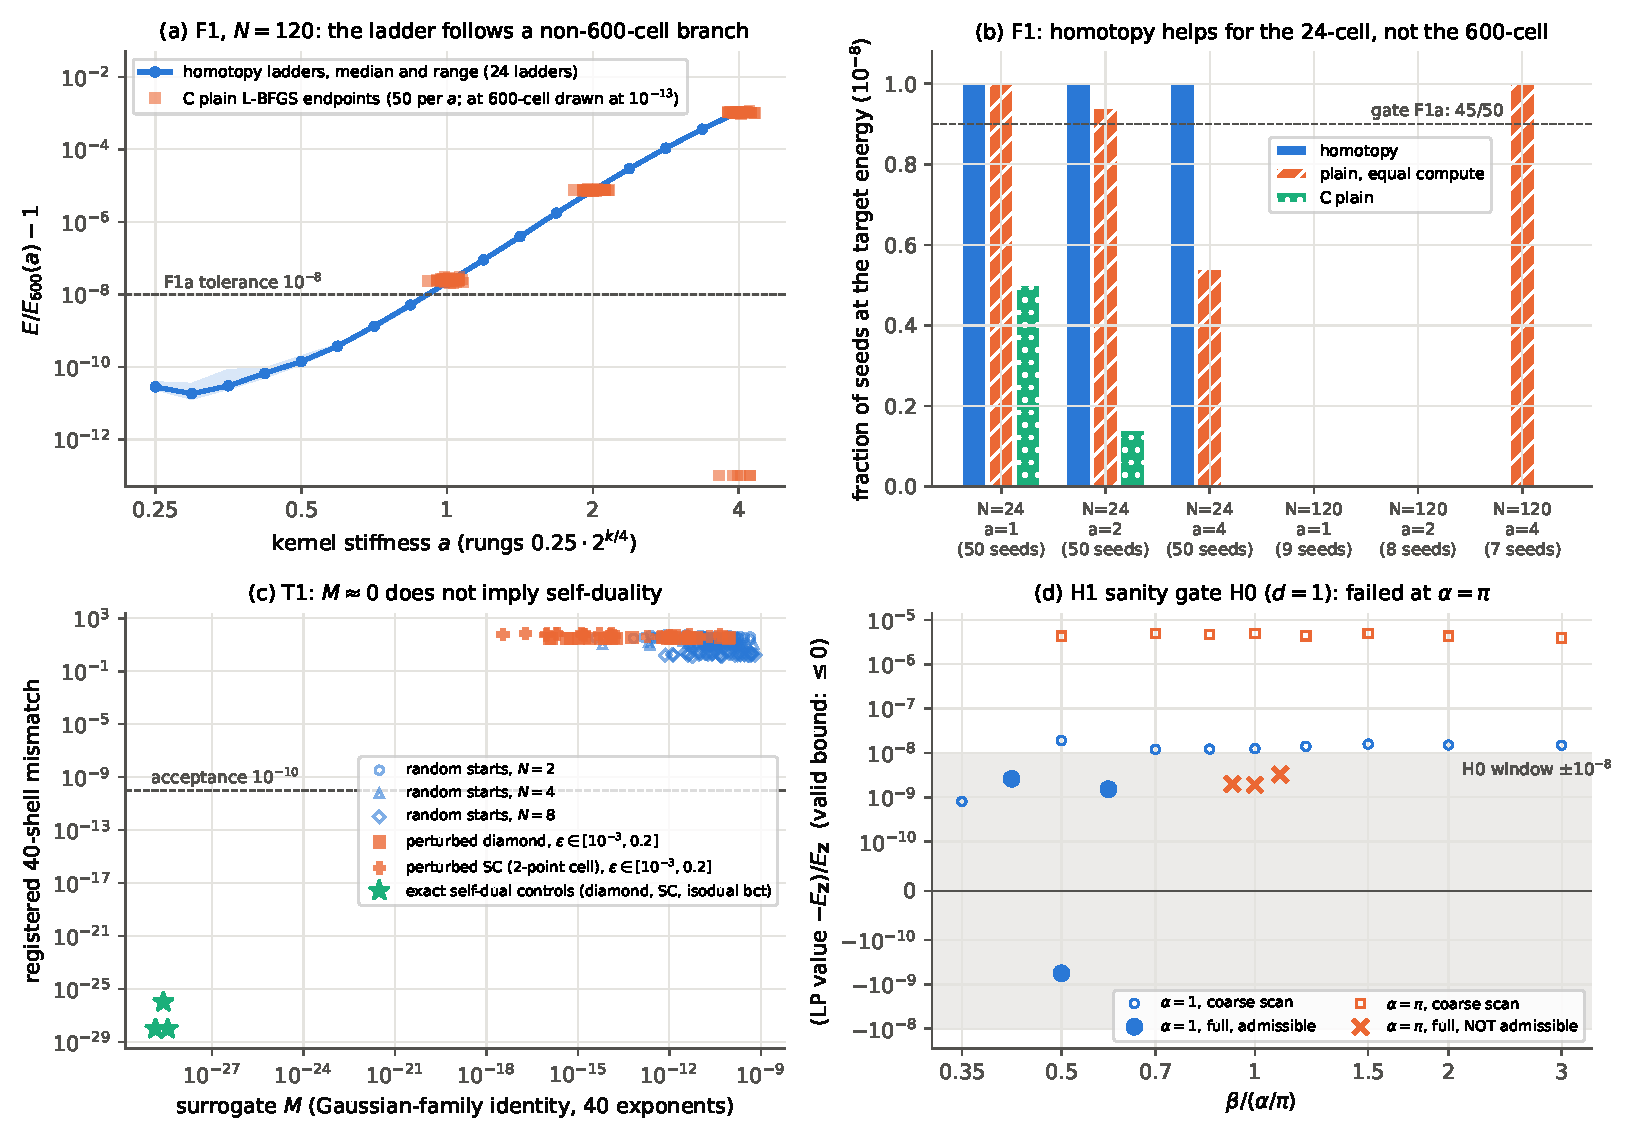
\includegraphics[width=0.98\textwidth]{figs_companion5/fig_round2.pdf}\\[2pt]
{\footnotesize Round~2. (a) F1, $N=120$: relative energy above the 600-cell along the $\alpha$-ladders (line: median; band: range)
and C's plain endpoints at $a=1,2,4$ (squares; runs that reach the 600-cell are drawn at $10^{-13}$). (b) Fraction of seeds reaching
the target energy: homotopy, plain L-BFGS with restarts at equal compute, and C's plain runs at the same seeds. (c) T1: surrogate
value against the registered shell mismatch for random starts, perturbed positive controls and the exact controls. (d) H1 sanity
gate in $d=1$: LP value minus $E_{\mathbb Z}$ (a valid bound is $\le0$) over the $\beta$ scan; crosses are full-setting solutions
that miss the admissibility tolerance.}
\end{center}
\subsection{F1: homotopy in $\alpha$ against the proved control}
Same $N=120$ points on $S^3$ and kernels $e^{-ad^2}$ as in C; from C's random start at the same seed, L-BFGS to convergence at
$a_0=0.25$, then a geometric ladder of ratio $2^{1/4}$ to the target (rungs 8, 12, 16 for $a=1,2,4$), warm-started and with C's
optimiser settings. Gate F1a: $\ge45/50$ seeds within $10^{-8}$ (relative) of $E_{600}$ \emph{and} minimum chord within $10^{-6}$ of
$2\sin(\pi/10)$. Gate F1b: plain L-BFGS from the same start with restarts, hard-capped at the homotopy's number of gradient
evaluations ($\approx7$--$9.5\times10^4$), must \emph{not} also reach $\ge45/50$ at $a\in\{2,4\}$.
\begin{center}\small
\begin{tabular}{lccccc}\toprule
$a$ & homotopy at 600-cell & plain, equal compute & C plain (same seeds) & homotopy end, rel.\ excess & gradient evaluations\\\midrule
1 & F1H1 & F1P1 & F1C1 & F1X1 & F1N1\\
2 & F1H2 & F1P2 & F1C2 & F1X2 & F1N2\\
4 & F1H4 & F1P4 & F1C4 & F1X4 & F1N4\\\bottomrule
\end{tabular}
\end{center}
\textbf{F1a fails at every $a$.} The rung-by-rung record locates the failure: already at $a_0=0.25$ the converged state is
$3\times10^{-11}$ above $E_{600}$ and yet is not the 600-cell (one ladder re-run with chords recorded, \texttt{F1/supp\_rung\_chords.py}, seed 0: converged, minimum chord $0.237$ against $0.618$, distance-spectrum deviation $0.38$), and the excess then grows smoothly along the ladder
($2\times10^{-8}$ at $a=1$, $7\times10^{-6}$ at $a=2$, $10^{-3}$ at $a=4$) --- the same excesses as C's trapped plain runs. The soft
kernel does not select the 600-cell; it selects a family of nearby minima that the ladder then follows. Seven to nine of the 17
rungs stop at C's 8\,000-iteration cap, so the soft rungs are not fully converged; the registered settings were kept. At $a=4$
plain L-BFGS \emph{with restarts} at equal compute finds the 600-cell in F1P4 seeds: the per-run success rate of fresh restarts is
F1RATE (completed runs only; the budget-truncated last run of each seed is dropped, a small survivorship bias), against 6/50
in C. A separate unregistered check with 40 fresh seeds (\texttt{F1/fresh\_plain\_a4.py}) gives F1FRESH. F1PTEST; F1CREPRO.

Control $N=24$ (50 seeds): the homotopy ends at the 24-cell energy in 50/50 starts at every $a$ (44/50 also match the chord at
$a=1$, where six end at the 24-cell energy to $10^{-8}$ with a minimum chord $1$--$2\times10^{-6}$ from 1, just outside the
$10^{-6}$ tolerance --- incomplete convergence, not a different configuration), against C's plain 25, 7, 0 of 50 and plain
with restarts at equal compute 50, 47, 27 of 50; it never goes below the 24-cell. So the homotopy \emph{does} help at $N=24$, a
configuration known not to be universally optimal, and does not at $N=120$, where the target is proved.

\textbf{Consequence (registered stop rule).} F1a failed at every $a$; the three-dimensional structure searches of this programme
(B, T2, T1) are declared unreliable, and their negatives are read only as ``no counterexample found with an unreliable search''.

\subsection{T2: Gaussian mixtures across the self-dual point}
Kernel $e^{-a_1r^2}+\lambda e^{-a_2r^2}$, $(a_1,a_2)\in\{(\pi/2,2\pi),(\pi/4,4\pi),(2,5)\}$; $\lambda^*$ (where $E_{\rm FCC}=E_{\rm BCC}$)
by bisection to $10^{-12}$, then $\lambda\in\lambda^*\{0.9,0.97,1,1.03,1.1\}$; Experiment B's engine unchanged except for an appended
mixture class (bit-identical on the stored references). For $a_1a_2=\pi^2$ the mixture with $\lambda=(\pi/a_1)^{3/2}$ is exactly
self-dual ($\hat f=f$); the bisection recovers $\lambda^*=2\sqrt2$ (to $1.9\times10^{-12}$) and $8$ (to $2.3\times10^{-10}$; the
limit is double-precision cancellation, since the FCC--BCC difference of the $a_2=4\pi$ term is only $4.8\times10^{-7}$ against
energies of order 3.5). Search: $N\in\{2,4,8,12,16\}$ with round~1's restart counts, 5\,100 restarts in
75 cells. \textbf{Gate T2: 0 candidates}; no cell has anything below the best reference lattice (most negative
relative difference $-1.9\times10^{-15}$, i.e.\ ties), and in 14 cells (pair $(\pi/4,4\pi)$, $N\ge8$) the lowest energy found is
above it by up to $3.7\times10^{-13}$ relative. The FCC/BCC crossover of the mixture kernels, including the two exactly self-dual ones, is crossed without
any intermediate non-lattice structure for $N\le16$. Hit fractions are 0.75--1.00 at $\lambda^*$ (FCC and BCC are then one
target) and 0.33--0.72 elsewhere, as in round~1. Remark: a fixed-density cell with $N\le16$ is not expected to represent the two-density
coexistence that CKS list as the lowest known energy at $\alpha=\pi$ ($4\times10^{-6}$ below the pure lattices; our engine's $E_{\rm FCC}(\pi)$ is
$4.1\times10^{-6}$ above their coexistence energy, consistent), so T2 says nothing about coexistence.

\subsection{T1: formally self-dual configurations at $\alpha=\pi$}
Definition as implemented (radial form of~\cite{CKS09}, Sec.~VI, at density 1, $Q=P$): the pair-difference measure of $P$ (weights
$1/N$) equals its structure-factor measure on $\Lambda^*$ (weights $|S(w)|^2/N^2$; the pre-registration wrote $|S|^2/N$, the
Poisson-consistent normalisation is $N^2$). Detector: the first 40 non-zero shells of each side, mismatch $<10^{-10}$. Controls
before any search: diamond $1\times10^{-26}$ (positive), FCC$\leftrightarrow$BCC $0$, $\mathbb Z^3$ $0$, the isodual bct
$9\times10^{-30}$, HCP $3\times10^3$ and FCC with itself $3.5\times10^4$ (negative). Search: a smooth surrogate (the identity tested
on 40 Gaussians, exponents 0.94--10.5, relative residuals) minimised from 60, 60, 40 random starts for $N=2,4,8$, acceptance by
the registered detector. \textbf{0 accepted} (minimum mismatch 19.8, 7.7, 1.26; a polish stage minimising the shell residuals directly lowered
the $N=8$ minimum to 0.30). The grouping tolerance ($10^{-6}$) and weight floor ($10^{-8}$) of the detector are implementation
choices, not registered.

\begin{failbox}
\textbf{Why the T1 negative is uninformative} (diagnostics added after the run, unregistered). (i) The best records have surrogate
$\sim10^{-15}$ while their pair and structure-factor measures visibly differ (L1 distance of the cumulative distributions 0.7--2.4,
0 for diamond). The identity is analytic in $\alpha$, so exact vanishing on an interval would force equality; what fails is
numerical: 40 sampled exponents with relative residuals $\sim10^{-8}$ admit configurations whose measures differ at $O(1)$ (the
best $N=2$ record has relative residual $1.2\times10^{-10}$ at $\alpha=0.3$ but $3\times10^{-3}$ at $\alpha=30$) --- the
problem is ill-conditioned. (ii) From diamond and from $\mathbb Z^3$ written as a 2-point cell, perturbed by $10^{-3}$--$0.2$, the
minimiser ends at surrogate $\le10^{-10}$ in 50/50 cases and is accepted in \textbf{0/50}. At $\varepsilon=10^{-3}$ the
\emph{unminimised} perturbed diamond already has surrogate $3.6\times10^{-11}$ (shell mismatch 30.5): the surrogate cannot resolve a
$10^{-3}$ displacement from the known solution, so the minimiser has nothing to return along. (iii) The detector is exact on the
controls but discontinuous: under perturbation diamond's systematically absent reflections reappear in the structure-factor
measure with weights $<5\times10^{-5}$ (above the $10^{-8}$ floor), have no counterpart in the pair measure, and shift the
shell-by-shell comparison (mismatch $\sim30$). The end states are nevertheless genuinely not self-dual (relative residual
$1.5\times10^{-5}$ at $\alpha=30$, CDF distance 0.022 for the $\varepsilon=10^{-3}$ case). T1 therefore reports a method
failure, not an absence of formally self-dual configurations below FCC/BCC. A usable version needs an identifying objective or an
algebraic enumeration of the CKS constructions.
\end{failbox}

\subsection{H1: the two-point LP gap}
Cohn--Kumar bound~\cite{CK07} in the periodic form $E_g(P)\ge\hat f(0)-f(0)$ for radial $f\le g$ off the origin with $\hat f\ge0$ (the registered transcription from~\cite{CK07} was not made; the statement
was derived and its proof checked, \texttt{H1/RESULTS.md}, a deviation); ansatz $\hat f(y)=e^{-\pi|y|^2/\beta}p(|y|^2)$, $\deg p\le30$, in the Laguerre eigenbasis
of the Fourier transform; HiGHS LP with cutting planes, 40-digit tail certificates, and an admissibility tolerance (polished violation
$\le5\times10^{-9}$) fixed in code before the run --- on file timestamps, not a commit --- and not in the pre-registration. Sanity gate H0 in $d=1$, where $\mathbb Z$ is universally optimal and the bound is sharp:
at $\alpha=1$ the bound is $0.7726372068$ against $E_{\mathbb Z}=0.7726372048$ ($+2\times10^{-9}$, inside the registered $10^{-8}$,
and also a measure of the discretisation error, since a valid bound cannot exceed $E_{\mathbb Z}$); at $\alpha=\pi$ the
full-setting values are $+1.6$ to $+2.8\times10^{-10}$ from $E_{\mathbb Z}$, inside the registered $10^{-8}$, but none meets the
code's admissibility tolerance (violations $2$--$5\times10^{-8}$). \textbf{H0 failed under the code's admissibility tolerance
(not registered); the stop then followed the registered rule}, and the $d=3$ gap has no value in this paper. The registered
$10^{-8}$ and the code's $5\times10^{-9}$ measure the same discretisation error from two sides (the $\alpha=1$ value is itself
$2\times10^{-9}$ \emph{above} $E_{\mathbb Z}$); part of the failure may also be a limit of the $K=30$ ansatz rather than of
certification. The H1
thresholds ($10^{-6}$, $10^{-3}$) lie far above this $10^{-8}$ level, so a re-registered run with exact (rational or
sum-of-squares) non-negativity certificates would probably be informative; it is left open.

\subsection{Round 2 deviations}
F1: the run was interrupted after 6 of 50 seeds when the launching session was compacted and resumed for seeds 6--49 with the
same code and single-threaded BLAS; \texttt{run\_F1.py} replaces C's energy evaluator by an equivalent
Gram-matrix form, asserted equal to $10^{-12}$ before every run (an oversubscribed first resume was stopped after 8 minutes, before any record). By then F1a
had already failed at every $a$ (6 misses each, more than the 5 allowed). The N$=24$ control completed in the first session.
T2: mixture class appended; diamond and A15 added for information. T1: the $N^2$ normalisation; surrogate run~1 (16 Gaussians,
absolute residuals) uninformative and discarded with records kept; run~2 start counts not registered (60/60/40); a typo in the
bct control fixed and rerun; an earlier draft and stale code comments in \texttt{expT1.py} and \texttt{selfdual.py}
misdescribed run~2's surrogate, corrected after a partial rerun reproduced 20 run-2 records bit for bit; detector tolerances not
registered. H1: the admissibility tolerance was fixed in code before the run but not in the
pre-registration (file timestamps only); \texttt{lp\_bound.py} was touched during the run, a docstring-only change (compiled
bytecode identical); tail grids and certificates added; the bound was derived rather than transcribed. All four were written up after a context compaction of the session that
launched them, from the records and logs only.


\section{Version 2: H1$'$, two-point LP values reproduced numerically}\label{sec:h1p}
\emph{Added in version~2 (\texttt{exploration/exciton/three\_d/H1p/}, pre-registration \texttt{d668109}, amendments A1
\texttt{83a3500} and A2 \texttt{968dd32}, code frozen at \texttt{91b1a97}, results \texttt{350bc74}, after review \texttt{6f5a1cb}).}
A literature check before re-registering found that H1's $\alpha=\pi$ question is answered in~\cite{CdCI16} (Table~1.1: two-point
bound $0.08643481\ldots$, $0.15959526\ldots$, $0.22321782\ldots$ in $d=1,2,3$; record $0.23153532\ldots$ in $d=3$). H1$'$ was
registered to reproduce these values with \emph{rigorous} certificates (exact rational positivity of $\hat f$, interval
arithmetic for $f\le(1+\tau)g$, bound $(\hat f(0)-f(0))/(1+\tau)$ by the Cohn--Kumar proposition as stated
in~\cite{CdCI16} for arbitrary configurations). Development at non-gate parameters showed this does not work with our LP: the
double-precision optimum is a degenerate face resolved only at its first few contacts (at $d=1$, $\alpha=2$ the LP controls $f$ only up to
$x\approx3$; beyond, $(f-g)/g$ reaches $3\times10^{43}$ at $x=8$), an exchange step chosen in amendment~A1 is
ill-posed for such a face, and a high-precision Newton polish stalled. Amendment A2, committed before any gate run, replaced certification by a \textbf{numerical, non-rigorous}
reproduction: H1's code unchanged, $K=30$ and $K=40$ (gate on $K=40$), solutions accepted if residual violations are
$\le10^{-7}$, two-sided windows.
\begin{center}\small
\begin{tabular}{llllll}\toprule
gate & $d$ & $\alpha$ & value ($K=40$) & reference & verdict\\\midrule
V1 & 1 & 1 & $0.7726372059$ & $E_{\mathbb Z}=0.7726372048$ ($+1.4\times10^{-9}$ rel.) & pass\\
V1 & 1 & $\pi$ & $0.0864348114$ & $E_{\mathbb Z}=0.0864348112$ ($+2.7\times10^{-9}$ rel.) & pass\\
V2 & 2 & $\pi$ & $0.1595952701$ & published $0.15959526\ldots$, window $[0.15959525, 0.15959528]$ & pass\\
V3 & 3 & $\pi$ & $0.2232178249$ & published $0.22321782\ldots$, window $[0.22321781, 0.22321784]$ & pass\\\bottomrule
\end{tabular}\\[4pt]
\begin{tabular}{lllll}\toprule
$\alpha$ & value ($K=40$) & $E_{\rm FCC}$ & $E_{\rm BCC}$ & gap to the best lattice\\\midrule
2 & $1.011018287$ & $1.017616896$ & $1.015862816$ & $4.8\times10^{-3}$\\
4 & $0.07275645512$ & $0.07796767103$ & $0.07889601371$ & $6.7\times10^{-2}$\\
8 & $0.0003947635566$ & $0.0005032413016$ & $0.0006026980499$ & $0.216$\\\bottomrule
\end{tabular}
\end{center}
\textbf{Reading.} The values are LP objectives, not bounds: they can exceed the true optimum by far more than the residual
violations (the $d=2$ value is $3.1\times10^{-9}$ above the triangular-lattice energy, which no valid bound can be, with a residual
of $9\times10^{-11}$). $d=1$ and $d=3$ match the printed 8 digits (for $d=3$, with the observed slack of up to $35\times$ the residual, an excess
of order $2\times10^{-8}$ cannot be excluded, comparable to the window); $d=2$ passes only through the registered window. At $K=30$ the
$d=3$ value would miss V3 by $4.6\times10^{-7}$; $K=50$ was not run. The gaps exceed the registered $10^{-3}$ at all three $\alpha$, as predicted: numerically,
at $K\le40$ and with the best lattice as reference, two-point bounds do not settle the three-dimensional Gaussian-core question at
$\alpha=2,\pi,4,8$; at $\alpha=2$ the reading assumes no non-lattice state lies more than about $0.4\%$ below BCC, which we did not check.
Choosing $\beta$ by the largest value favours the most-violating accepted solution, and at $\alpha=8$ the $\beta$ optimum is not
bracketed (irrelevant at a $22\%$ gap). This is what the literature value at $\alpha=\pi$ led us to expect, and the $\alpha=2,4,8$ numbers are new only
in the sense that we did not find them published. Rigorous certification at $10^{-8}$ remained open in version~2; version~3 supplies it with a different, interval-certified construction, after a post-hoc re-check that closed a defect in its certificate code (Sec.~\ref{sec:h1pp}). The hostile review found no
blocking item; its corrections (a residual, the ``8 digits'' claim for $d=2$, the size of the slack, prior knowledge of the $K=30$
$d=1$ outcomes from H1, the $\alpha=2$ reference caveat) are applied here and in \texttt{H1p/RESULTS.md}.

\section{Version 3: H1$''$ and H1$'''$, certified two-point bounds}\label{sec:h1pp}
% Version 3 section (H1''), included from exciton_fluid_gated_V.tex. Numbers: exploration/exciton/three_d/H1pp/summary.json.
\emph{Added in version~3 (\texttt{exploration/exciton/three\_d/H1pp/}, pre-registration and frozen code \texttt{b1d2de5}).}
Version~2 left rigorous certification open. Its obstacle was arithmetic: with the constraint rewritten as $f/g\le1$, the
$O(1)$ terms of $f$ must cancel to the size of $g$ ($10^{-14}$ at the first contacts), about 23 significant digits, which
double precision does not have. H1$''$ is the different construction that the version~2 development notes called for.

\textbf{Method.} Same ansatz as H1 ($\hat f=e^{-t/2}Q(t)$, $f=\beta^{d/2}e^{-u/2}R(u)$, Laguerre coefficients $c_k$, odd effective
degree $39$ at $K=40$). (i)~The LP is solved by a primal--dual interior-point method in 256-bit arithmetic (python-flint arb
midpoints), with rows $f/g\le1$ up to $g=10^{-12}$, $R\le-10^{-12}$ beyond, $Q\ge0$ on $t\in[0,\infty)$ (log grid far out).
(ii)~Cutting planes come from \emph{exact} objects: after each round the coefficients are made dyadic-rational and the real roots
of $R'-\kappa R$ (which contain every local maximum of $f/g$), of $R$ beyond the last contact and of $Q$ are isolated
rigorously; violated regions receive rows. (iii)~Every round's coefficient vector is \emph{certified} in interval arithmetic:
$R<0$ beyond its largest real root; $f/g\le1+\tau_0$ on the rest by bisection with Taylor-shift enclosures; $\hat f+\delta
e^{-\pi|y|^2/(\lambda\beta)}\ge0$ (a Gaussian lift, $\lambda\ge1/b$, which adds at most $\delta(\lambda\beta)^{d/2}$ to $f/g$), so
that $f_{\rm tot}\le(1+\tau)g$ and the Cohn--Kumar proposition in the form of~\cite[Prop.~2.2]{CdCI16} gives the certified
bound $B=[\hat f(0)+\delta-f(0)-\delta(\lambda\beta)^{d/2}]/(1+\tau)$, whose lower interval end is reported. The best
certified $B$ over at most 25 rounds is kept (any certified vector is a valid bound, so the choice cannot invalidate it).
Development was at non-gate parameters only and found four defects of our own before registration (a real-root filter that
saw no roots, a $6\times10^{-7}$ spike of $f/g$ at a contact missed by a 20\,000-point grid, row pruning that made violations
recur, too narrow a lift); they are listed in \texttt{H1pp/DEV\_NOTES.md}.

\textbf{H1$''$ results ($K=40$, gate on V3).} V1 ($d=1$, $\alpha=1$ and $\pi$) certified $B$ within $6.7\times10^{-13}$
and $2.3\times10^{-11}$ (relative) of $E_{\mathbb Z}$; V2 ($d=2$) within $7.6\times10^{-12}$ of $E_{A_2}$: pass. \textbf{V3
($d=3$, $\alpha=\pi$) failed}: certified $B=0.2232177894732$, $3.05\times10^{-8}$ below the published $0.22321782$, outside the
registered $10^{-8}$ window. By the registered stop rule the $\alpha=2,4,8$ runs were reported as gated only, and the cause was left
undetermined. A machine reboot killed seven running jobs after about $6.5$\,h; the thirteen unfinished runs were relaunched
unchanged (no result was selected between launches), which is why the next round's driver checkpoints.

\textbf{H1$'''$: larger $K$ only} (\texttt{three\_d/H1ppp/}, pre-registration and frozen code \texttt{1e50f4b}). The method,
row grids, certificate, $b$ values and gate window of H1$''$ are unchanged; only $K=50$ (gate) and $K=60$ (V3 only, reported).
The registered evaluator turned out to be an unmodified copy of H1$''$'s, which reads only $K=40/30$ records; a replacement
applying the same criteria was committed (\texttt{162dfc3}) while the runs were in flight and before any record existed, after
intermediate per-round values in the logs had been seen (\texttt{H1ppp/DEVIATIONS.md}). The five runs ran uninterrupted
(10\,h at most). Certificates: $\tau\le1.1\times10^{-13}$, Gaussian lift $\delta\le2\times10^{-28}$.
\begin{center}\small
\begin{tabular}{lllll}\toprule
case & $K$ & certified $B$ & reference & verdict\\\midrule
V3 ($\alpha=\pi$) & 40 (H1$''$) & $0.2232177894732$ & published $0.22321782$; $-3.05\times10^{-8}$ & fail\\
V3 ($\alpha=\pi$) & \textbf{50} & $0.2232178193590$ & $-6.4\times10^{-10}$; window edge $0.22321781$ & \textbf{pass (gate)}\\
V3 ($\alpha=\pi$) & 60 & $0.2232178245495$ & $+4.5\times10^{-9}$ & reported\\\midrule
$\alpha=2$ & 50 & $1.011018246684$ & $E_{\rm BCC}=1.015862816$ & $G=4.77\times10^{-3}$\\
$\alpha=4$ & 50 & $0.07275645543946$ & $E_{\rm FCC}=0.07796767103$ & $G=6.68\times10^{-2}$\\
$\alpha=8$ & 50 & $0.0003947602893426$ & $E_{\rm FCC}=0.0005032413016$ & $G=0.216$\\\bottomrule
\end{tabular}
\end{center}
\textbf{Reading.} The gate passes at $K=50$ with a margin of $9.4\times10^{-9}$, so the $\alpha=2,4,8$ values are registered
results: \emph{certified} lower bounds on the Gaussian energy per point of every unit-density configuration in $\mathbb R^3$,
$0.48\%$, $6.7\%$ and $21.6\%$ below the best lattice. Version~2's numerical statement --- two-point bounds at this degree do not
settle the three-dimensional Gaussian-core question at $\alpha=2,4,8$ --- now holds with rigorous bounds (with the same
caveat at $\alpha=2$: it assumes no non-lattice state more than about $0.4\%$ below BCC). The V3 value rises monotonically with
$K$ ($+3.0\times10^{-8}$ from 40 to 50, $+5.2\times10^{-9}$ from 50 to 60), so H1$''$'s shortfall is accounted for by
truncation at $K=40$; the other candidates (snapped $b$, row margin) were not tested and are not needed. That $K=60$ exceeds
$0.22321782$ is consistent with the published digits being truncated. The registered prediction (gate passes, $G>10^{-3}$ at
all three, values within $10^{-6}$ relative of H1$'$'s) failed in its last part at $\alpha=8$: the certified value is
$8.3\times10^{-6}$ below H1$'$'s uncertified LP objective, which overshot. Not shown: convergence in $K$, the best two-point
bound at $K=50$ ($b$ was not re-optimised), anything about three-point or semidefinite bounds.


\section{What this does and does not show}
\begin{itemize}[leftmargin=1.2em,itemsep=1pt]
\item The 3D Bravais problem for completely monotone kernels is settled numerically on our grids (FCC or BCC, exact Gaussian
crossover at $\pi$); nothing new is claimed there.
\item No non-Bravais structure beats the references for pure kernels up to 16 points per cell; this is an absence of counterexample
with a search whose reliability is itself measured (B1 near-misses, C failures) and that round~2's stop rule, as we read it, declares unreliable.
\item The ``lift and project'', ``branes as walls'' and ``curved space'' pictures are now each attached to a negative or marginal
measurement (papers IV, this paper); the ``KK tower'' picture is a real and modest evaluator gain; the ``T-duality'' picture is a
correct explanation of a negative fact.
\item Round~2 adds no positive result. Its main product is a measured limit: with our optimisers, a homotopy in the kernel does
not find a proved optimum on $S^3$ (the 600-cell) that plain restarts find at $a=4$, the formal-duality search cannot distinguish a known
formally self-dual structure from nearby non-self-dual ones, and our original LP code is not certified at the $10^{-8}$ level (version~2 reproduces published values numerically with it, Sec.~\ref{sec:h1p}; version~3 uses a new, interval-certified construction, Sec.~\ref{sec:h1pp}).
These are statements about our methods, not about the Gaussian-core conjecture.
\item Version~2 (H1$'$) adds a reproduction, not a result: our LP code matches published two-point values numerically, and
the $d=3$ gaps at $\alpha=2,4,8$ are of the size the literature led us to expect; nothing is certified.
\item Version~3 (H1$''$, H1$'''$) certifies the bound values: rigorous two-point lower bounds at $K=50$ (degree $49$),
validated against the published $d=3$, $\alpha=\pi$ value after a failed attempt at $K=40$. The gaps to the best lattice are
upper estimates of the true two-point gap at this degree; that two-point bounds cannot settle these cases is not certified (it
would need a dual certificate). Rigour here rests on the frozen certificate plus an independent re-check that closed a defect
found in review. Nothing here proves or refutes FCC/BCC optimality.
\item Nothing here involves the planar lattice theorem of \texttt{openai/math}, which remains AI-generated and unrefereed, nor any
claim about excitons.
\end{itemize}

\section{Process and deviations}\label{sec:process}
Round~1 deviations: B restart counts reduced (100/100/60/40/40); A reruns after bugs with records kept; C1 operationalised as
$\ge45/50$ and the $a=1$ rerun added after review; D's comparator defined by the run's author before running but not registered;
L3's pre-registration untracked at run time; L3 annulus G2 cases run twice with the second overwriting the first; a timing check on
an uncounted seed. L1: mpmath reference at 10 of 160 points; first run discarded for a reference bug. Round~2 deviations are listed
with the results. All raw records, analysis scripts and the reviews (round~1, round~2, F1, in version~2 H1$'$, in version~3 H1$'''$ with its re-check script) are in the repository (the H1$''$ review's corrections were applied in commit \texttt{25eecce}, but the review text itself was not saved); the independent review of round~1
(\texttt{docs/designs/EXCITON\_FLUID\_VERIFIER\_NOTES\_review\_3d.md}) recomputed every headline number from the records and asked for
the wording changes applied here (D ``not met at matched cost'', B1 ``strictest reading'', C $a=1$ resolved by rerun).

\begin{thebibliography}{99}\small
\bibitem{CallensI} X. Callens, \emph{Gated exciton fluids}, Zenodo, \url{https://doi.org/10.5281/zenodo.23294615} (2026).
\bibitem{CallensII} X. Callens, \emph{Gated exciton fluids II}, Zenodo, \url{https://doi.org/10.5281/zenodo.23297479} (2026).
\bibitem{CallensIII} X. Callens, \emph{Gated exciton fluids III}, Zenodo, \url{https://doi.org/10.5281/zenodo.23298292} (2026).
\bibitem{CallensIV} X. Callens, \emph{Gated exciton fluids IV}, Zenodo, \url{https://doi.org/10.5281/zenodo.23302787} (2026).
\bibitem{CdCI16} H. Cohn, M. de Courcy-Ireland, The Gaussian core model in high dimensions, arXiv:1603.09684 (v6, 2018).
\bibitem{CK07} H. Cohn, A. Kumar, Universally optimal distribution of points on spheres, \emph{J. Amer. Math. Soc.} 20 (2007) 99--148.
\bibitem{CKS09} H. Cohn, A. Kumar, A. Sch\"urmann, Ground states and formal duality relations in the Gaussian core model, arXiv:0911.2169 (2009).
\bibitem{CK08} H. Cohn, A. Kumar, Counterintuitive ground states in soft-core models, \emph{Phys. Rev. E} 78 (2008) 061113, arXiv:0811.1236.
\bibitem{CCEK07} H. Cohn, J. H. Conway, N. D. Elkies, A. Kumar, The $D_4$ root system is not universally optimal, \emph{Exp. Math.} 16 (2007) 313--320.
\bibitem{CKMRV22} H. Cohn, A. Kumar, S. D. Miller, D. Radchenko, M. Viazovska, Universal optimality of the $E_8$ and Leech lattices and interpolation formulas, \emph{Ann. of Math.} 196 (2022) 983--1082.
\bibitem{RV19} D. Radchenko, M. Viazovska, Fourier interpolation on the real line, arXiv:1701.00265.
\end{thebibliography}
\end{document}
